\documentclass[tikz]{standalone}
\usepackage{fontspec}
\renewcommand*{\familydefault}{\sfdefault}
\usepackage{standalone}
\usepackage{amssymb}
\usetikzlibrary{arrows.meta, decorations.pathreplacing, shapes.geometric}
%\usetikzlibrary{positioning,fit,shapes.geometric,fadings,bayesnet}

\begin{document}

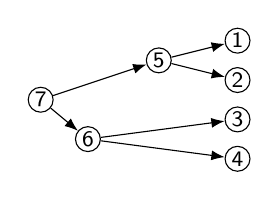
\begin{tikzpicture}
[font=\footnotesize, label distance=0 cm, inner sep=0.5 pt,
%every node/.style={anchor=center},
every node/.style={draw, inner sep=0 pt, minimum size=9 pt, circle, fill=none}
]

\path
coordinate (v1) at (0,0)
coordinate (v5) at (0,-0.25)
coordinate (v2) at (0,-0.50)
coordinate (v7) at (0,-0.75)
coordinate (v3) at (0,-1.00)
coordinate (v6) at (0,-1.25)
coordinate (v4) at (0,-1.50)
;

\coordinate (top) (0,0) ;

\path[draw]
foreach \x in {1,...,4}
{(v\x-|top.west) +(-0.0,0) node (V\x) {\x}}
(v5-|top.west) +(-1.0,0) node (V5) {5}
(v6-|top.west) +(-1.9,0) node (V6) {6}
(v7-|top.west) +(-2.5,0) node (V7) {7}
;

% draw phylogeny
\begin{scope}[-Latex]
\draw (V7) -- (V5) ;
\draw (V5) -- (V1) ;
\draw (V5) -- (V2) ;
\draw (V7) -- (V6) ;
\draw (V6) -- (V3) ;
\draw (V6) -- (V4) ;
\end{scope}


\end{tikzpicture}

\end{document}
